\section{glist Strukturreferenz}
\label{structglist}\index{glist@{glist}}
{\tt \#include $<$linklist.h$>$}

Zusammengeh\"{o}rigkeiten von glist:\begin{figure}[H]
\begin{center}
\leavevmode
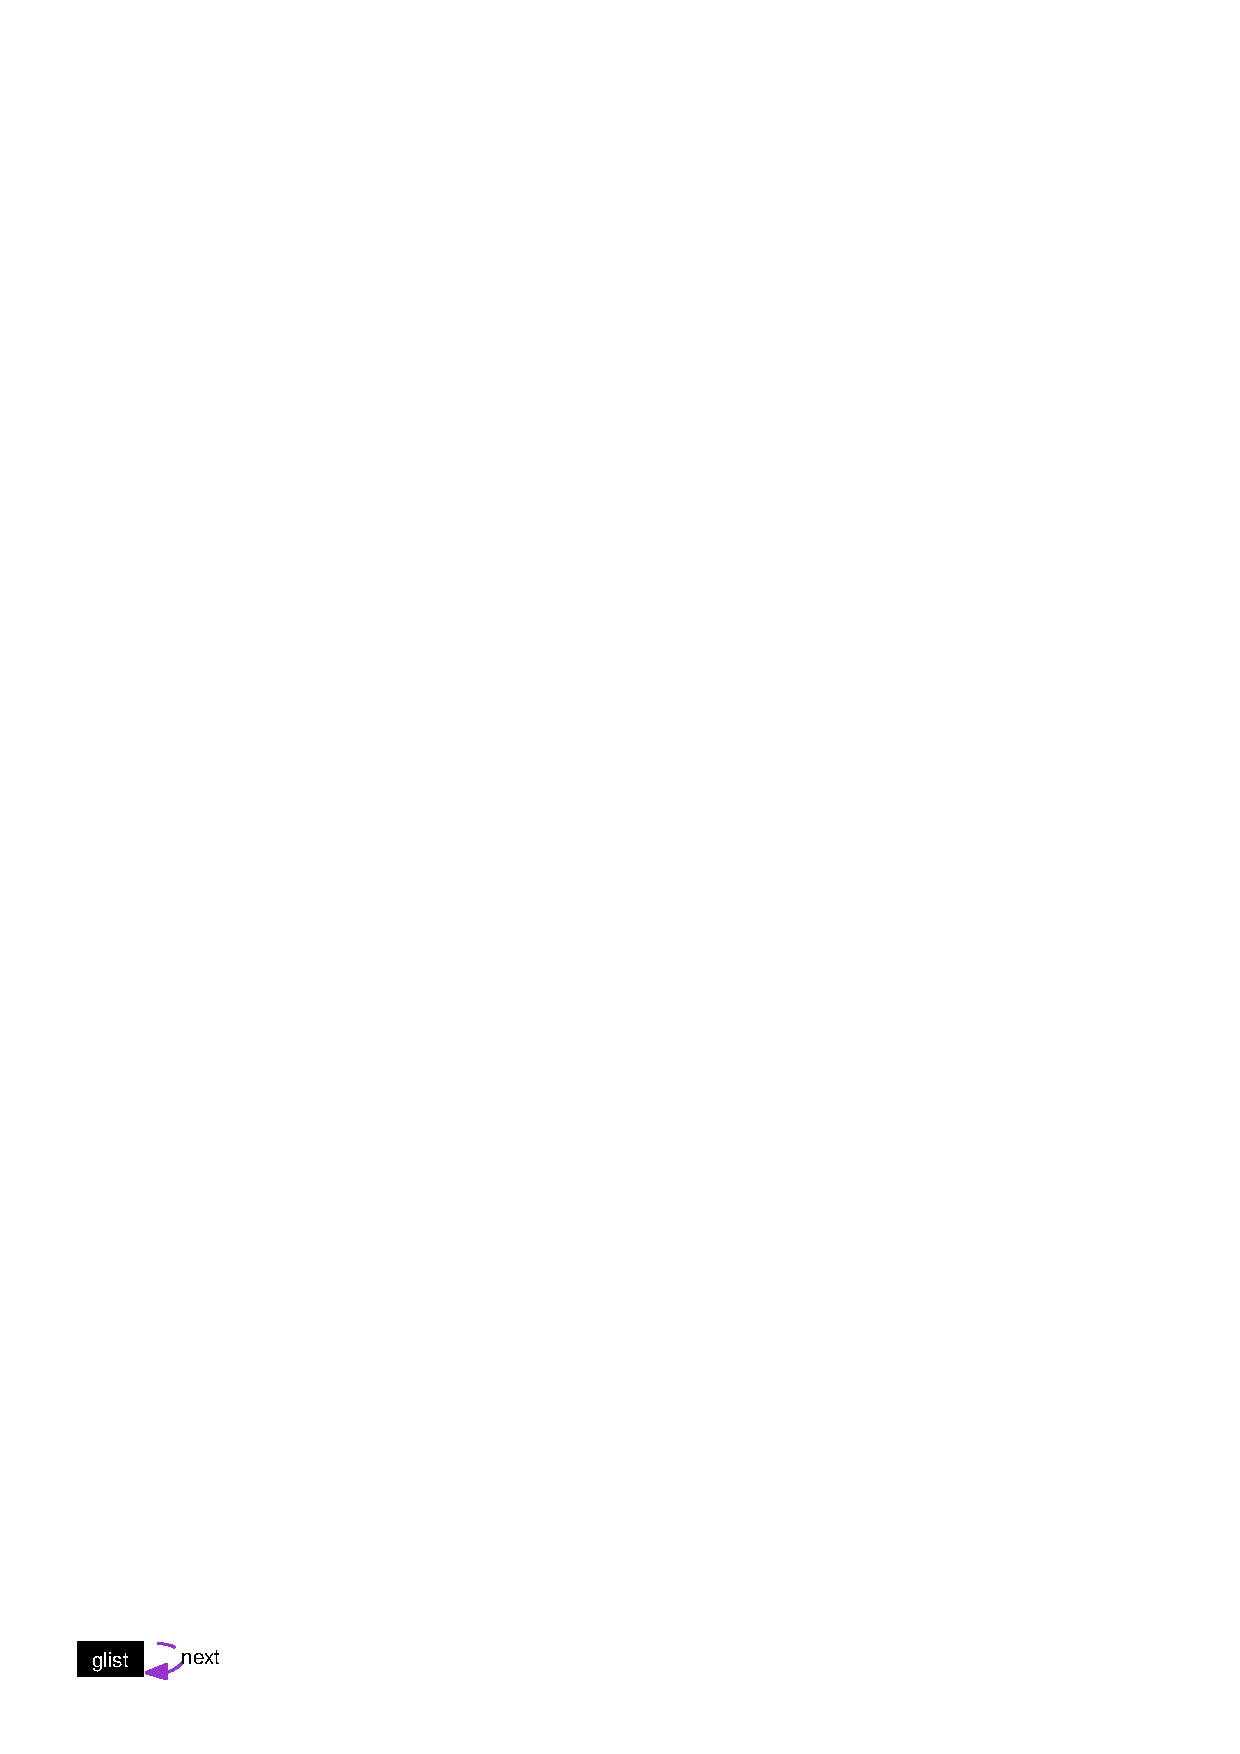
\includegraphics[width=54pt]{structglist__coll__graph}
\end{center}
\end{figure}
\subsection*{Datenfelder}
\begin{CompactItemize}
\item 
char {\bf string} [80]
\item 
char {\bf name} [80]
\item 
{\bf glist} $\ast$ {\bf next}
\end{CompactItemize}


\subsection{Ausf\"{u}hrliche Beschreibung}




Definiert in Zeile 8 der Datei linklist.h.

\subsection{Dokumentation der Datenelemente}
\index{glist@{glist}!name@{name}}
\index{name@{name}!glist@{glist}}
\subsubsection{\setlength{\rightskip}{0pt plus 5cm}char {\bf glist::name}[80]}\label{structglist_d3ebdbe9d3d9448d753a3aa95d232455}




Definiert in Zeile 9 der Datei linklist.h.

Wird benutzt von isinglist() und new\_\-glist().\index{glist@{glist}!next@{next}}
\index{next@{next}!glist@{glist}}
\subsubsection{\setlength{\rightskip}{0pt plus 5cm}struct {\bf glist}$\ast$ {\bf glist::next}}\label{structglist_fcbd6d229e8a0ea95ed0532927a3bf85}




Definiert in Zeile 10 der Datei linklist.h.

Wird benutzt von add\_\-glist(), del\_\-glist(), isinglist() und new\_\-glist().\index{glist@{glist}!string@{string}}
\index{string@{string}!glist@{glist}}
\subsubsection{\setlength{\rightskip}{0pt plus 5cm}char {\bf glist::string}[80]}\label{structglist_36312d3b785bc51f116bd01aa2a3cf20}




Definiert in Zeile 8 der Datei linklist.h.

Wird benutzt von isinglist() und new\_\-glist().

Die Dokumentation f\"{u}r diese Struktur wurde erzeugt aufgrund der Datei:\begin{CompactItemize}
\item 
oosalizer/{\bf linklist.h}\end{CompactItemize}
